\documentclass[11pt,a4paper]{article}
\usepackage[utf8]{inputenc}
\usepackage[german]{babel}
\usepackage{amsmath}
\usepackage{amsfonts}
\usepackage{hyperref}
\usepackage{booktabs}
\usepackage{setspace}
\usepackage{threeparttable}
\usepackage{amssymb}
\usepackage{graphicx}
\usepackage{fancyhdr}
\usepackage{icomma}
\usepackage{float}
\usepackage{pdfpages}
\usepackage{hyperref}
\usepackage[left=2.5cm,right=2.5cm,top=2cm,bottom=3.5cm]{geometry}
\title{DreamSwipe\\Tinder für Filme\vspace{10px}}
\author{Leon Gieringer, Robin Meckler,Vincent Schreck \\ \\ Studienarbeit \\ \\ \\}
\date{\today}

\begin{document}
\maketitle
\thispagestyle{empty}
\newpage
\pagenumbering{Roman}
\tableofcontents
\newpage
\pagenumbering{arabic}

\pagestyle{fancy}
\fancyhf{}
\setlength{\headheight}{35pt}
\lhead{DreamSwipe}
\rhead{Studienarbeit}
\cfoot{\thepage}
\newpage


\section{Einleitung}


\section{Motivation}


\section{Theoretische Grundlagen}


\subsection{Framework}
Hier steht mein Framework Text
\subsection{Language}
Hier steht mein Language Text.

\subsection{IDE}
Hier steht mein IDE Text.

\subsection{Database}
Hier steht mein Database Text.

\subsection{Firebase}
Firebase ist eine Backend-as-a-Service (BaaS) Plattform von Google für mobile oder Web-Anwendungen. 
Sie soll es dem Entwickler ermöglichen, einfacher und effizienter Funktionen auf verschiedenen Plattformen bereitzustellen stellt Tools und Infrastruktur zur Verfügung.
Mit dem Firebase SDK bietet die Plattform API Schnittstellen zu den jeweiligen Tools, welche direkt in die Anwendung integriert werden können, ohne dass serverseitiger Code dafür notwendig ist.
Die Firebase Inc. wurde 2011 von James Tamplin und Andrew Lee gegründet und letztendlich 2014 von Google übernommen.\footnote{\href{https://firebase.googleblog.com/2014/10/firebase-is-joining-google.html}{firebase.googleblog.com}, zuletzt aufgerufen am 03.05.2021}
Teile der SDK stehen seit der Google I/O 2017 unter der Apache 2.0 Lizenz, sind somit also Open-Source.\footnote{\href{https://opensource.googleblog.com/2017/05/open-sourcing-firebase-sdks.html}{opensource.googleblog.com}, zuletzt aufgerufen am 03.05.2021}\\
\\
Es existieren zwei Kostenmodelle für die Nutzung von Firebase: Ein kostenloses Modell \glqq Spark Plan\grqq und ein pay-as-you-go \glqq Blaze Plan\grqq . Das kostenlosen Modell beinhaltet die wichtigsten Tools, viele dieser Tools sind jedoch begrenzt durch beispielsweise Bandbreite oder Speicherplatz.
Der Pay-as-you-go Plan ist eine Erweiterung des kostenlosen Plans. 
Er bietet daher das Nutzen von Tools bis zu einem gewissen Limit kostenfrei an; darüber hinaus kostet es jedoch dann pro Nutzung.\\
\\
Ein Firebase Projekt ist die oberste Ebene in Firebase. 
Ein Projekt ist letztendlich ein \textit{Google Cloud Projekt}, welches mit speziellen Konfigurationsmöglichkeiten und Services ausgestattet ist. 
Es beinhaltet die Verknüpfung zu den einzelnen Anwendungen (also bspw. Android-, iOS- oder Webanwendung). Nun können variabel Tools, sog. Firebase products hinzugefügt werden. Diese Produkte lassen sich grundlegend in drei Kategorien einteilen. Die hier relevantesten werden im Folgenden besprochen.\cite{firebase2021}

\subsubsection{Firebase Authentifizierung}
Die Authentifizierung gehört zu den \glqq Build\grqq Produkten und bietet eine Token-basierte Nutzerauthentifizierung. 
Hierbei kann zwischen verschiedenen Anmeldeoptionen gewählt werden: klassisch mit E-Mail und Passwort, mit OAuth2.0 Integration für Social Media (Google, Facebook, Twitter, Github, ...) oder per Telefonnummer.
Jeder Nutzer erhält eine einzigartige ID und ein zugehöriges Nutzerobjekt in einer NoSQL Datenbank. Grundlegende Werte wie E-Mail Adresse oder Name können hier abgespeichert werden; zusätzliche Informationen müssen über einen weiteren Datenbank Service abgespeichert werden.
Für die Verwaltung eines Accounts bietet dieses Tool auch eingebaute E-Mail Aktionen an - bspw. Passwort zurücksetzen oder E-Mail Adresse bestätigen.\\
\\
Ein Firebase Nutzer Objekt repräsentiert den Account eines Nutzers, welcher sich von einer Anwendung aus beim zentralen Firebase Projekt angemeldet hat.
Die Instanz eines Firebase Nutzers ist somit unabhängig von der Authentifizierungsinstanz der Anwendung, also kann eine Anwendung mehrere Nutzer anmelden, jedoch kann sich auch ein Nutzer auf mehreren Anwendungen anmelden.
Ist ein Nutzer authentifiziert, erhält die Anwendung eine Referenz des Nutzers, welche so lange existiert, bis er wieder abgemeldet ist.\cite{firebase2021}

\subsubsection{Cloud Firestore}
\label{sec:firestore}
Als Datenbank Lösung bietet Firebase zwei unterschiedliche Produkte an: Cloud Firestore und Realtime Database.
Firestore ist hier neuer, jedoch ersetzt es Realtime Database nicht. \\
Cloud Firestore ist eine flexible und auf Skalierung ausgesetzte NoSQL Cloud Datenbank, welche unter anderem die Echtzeitsynchronisierung der Daten zwischen Anwendung und Server ermöglicht.
Zusätzlich zu REST und RPC APIs in iOS, Android und web SDKs ist Firestore auch in nativen Node.js, Java, Python und Go SDKs verfügbar.\\
\\

\begin{wrapfigure}{R}{0.4\textwidth}
	\begin{center}
		
\includegraphics[width=0.35\textwidth]{images/firestore_datastucture.png}
	\end{center}
	\caption{Datenmodell in Firebase \protect \footnotemark}
	\label{fig:firestore_data_structure}
\end{wrapfigure}
\footnotetext{Quelle: \cite{firebase2021}}

Das Datenmodell ist hierarchisch aufgebaut, wobei Daten in Dokumenten (documents) und Dokumente in Sammlungen (collections) gespeichert sind. 
Mithilfe von Sammlungen werden die Daten voneinander abgetrennt und hierüber können Abfragen erstellt werden.
Grundlegende Datentypen sind String, Integer und Boolean, jedoch können auch komplexe Datentypen wie Maps, Arrays oder Geopoints. Unter-Sammlungen und darin verstaute Dokumente sind ebenfalls möglich.\\
\\
Abfragen werden auf Dokumentenebene erstellt, damit nicht eine gesamte Sammlung aufgerufen werden muss.
Dies kann über direkte Sortierung, Filter und/oder Limitierung bzw. genaue Auswahl eines Dokumentes bewerkstelligt werden.
Bei einer Abfrage erhält man einen \textit{Data Snapshot}, wodurch über Änderungen in Echtzeit informiert und diese angezeigt werden können.
Damit es jedoch zu keinen fehlerhaften Daten führt, gelten hier atomare Eigenschaften für Transaktionen.
Eine Transaktion ist eine Folge von Datenbankanweisungen, welche entweder alle gemeinsam oder gar nicht ausgeführt werden. 
Eine Transaktion ist nur dann erfolgreich, wenn alle Anweisungen auf eine Datenbank vollständig geschlossen sind. 
Ist dies nicht der Fall, werden alle Anweisungen bis zum Stand vor der Transaktion rückgängig gemacht. Das nennt man Rollback.\\
\\
Die Sicherheit der Daten stellt Cloud Firestore für Mobil- und Webclient-Bibliotheken über die Firestore-Sicherheitsregeln her. Diese bieten sowohl Zugriffsverwaltung und -authentifizierung, jedoch könne auch Daten hiermit für die Konsistenz der Datenbank validiert werden. 
\medskip
\begin{lstlisting}[caption=Beschränkung des Zugriffs auf Dokumente der Sammlung \texttt{cities}, label=lst:firestorerules_basic]
	service cloud.firestore {
		match /databases/{database}/documents {
			match /cities/{city} {
				allow read, write: if request.auth != null;
			}
		}
	}
\end{lstlisting}
\medskip
Im Beispiel \ref{lst:firestorerules_basic} wird der Lese- und Schreibzugriff auf ein Dokument der Sammlung \texttt{cities} beschränkt. 
Nur falls der anfragende Nutzer eine valide Authentifizierung besitzt, erhält er Zugriff auf das angefragte Dokument. 
Diese simple Darstellung ist jedoch für den wirklichen Produktionseinsatz mit Vorsicht zu nutzen. 
Oftmals müssen \texttt{read} und \texttt{write} in detailliertere Vorgänge aufgeteilt werden. Ein \texttt{read} wird spezialisiert in \texttt{get} und \texttt{list}, wobei ein \texttt{write} in \texttt{create}, \texttt{update} und \texttt{delete} unterteilt werden kann.
Ein \texttt{list} ermöglicht es hierbei auf Sammlungen, also die einzelnen Dokumenten IDs lesend zuzugreifen, jedoch nicht auf die Daten einzelner Dokumente. Hierfür wird dann ein \texttt{get} benötigt. 
Mittels \texttt{create} erhält man Schreibzugriff auf nicht existierende Dokumente, durch \texttt{update} auf bereits vorhandene und Löschrechte ganzer Dokumente erhält man über den \texttt{delete} Operator.\\
\\
Sicherheitsregeln werden gleich dem Datenmodell hierarchisch aufgebaut und ermöglichen differenzierte Zugriffsbeschränkungen auf jeder Ebene.
In Codebeispiel \ref{lst:firestorerules_hierarchy} beinhaltet jedes Dokument (Stadt) der Sammlung \texttt{cities} eine Unter-Sammlung \texttt{landmarks}. Nun lässt sich der Zugriff auf beide separat regeln.
Bei der Sammlung \texttt{villages} hingegen wurde der rekursive Platzhalter verwendet. Hiermit sind Zugriffsregeln auf allen tieferen Ebenen gleich.
Beim Verschachteln von \texttt{match} ist der innere Pfad immer relativ zum äußeren.

Wichtig zu wissen ist hierzu noch, dass falls mehrere \texttt{allow} Ausdrücke auf eine Anfrage zutreffen, wird der Zugriff erlaubt sobald \textbf{eine} Bedingung wahr, also erfüllt ist.

\medskip
\begin{lstlisting}[caption=Hierarchische Zugriffsbeschränkung, label=lst:firestorerules_hierarchy]
	service cloud.firestore {
		match /databases/{database}/documents {
			match /cities/{city} {
				allow read, write: if <condition>;
				
				// Explicitly define rules for the 'landmarks' subcollection
				match /landmarks/{landmark} {
					allow read, write: if <condition>;
				}
			}
			match /villages/{document=**} {
				allow read, write: if <condition>;
			}
		}
	}
\end{lstlisting}
\medskip

Wie bereits oben besprochen können diese Regeln auch zur Validierung von Daten genutzt werden, damit die atomare Eigenschaft von Transaktionen bestehen bleibt.
Hierzu kann die \texttt{getAfter()} Funktion genutzt werden. 
Mit dieser kann man auf Zustand eines Dokumentes zugreifen und diesen validieren, nachdem einer Folge von Anweisungen ausgeführt, jedoch diese noch nicht auf der Firestore Datenbank abgeschlossen wurde.
Im Beispiel \ref{lst:firestorerules_validation} existieren zwei Sammlungen: \texttt{cities} und \texttt{countries}. 
Jedes \texttt{country} Dokument beinhaltet das Feld \texttt{last\_updated} um zu wissen, welche Stadt innerhalb eines Landes zuletzt aktualisiert wurde.
Hierzu wird in den Sicherheitsregeln nach jedem Schreibzugriff auf ein \texttt{city} Dokument gleichzeitig auch das Feld des zugehörigen Landes aktualisiert.\cite{firebase2021}
\medskip
\begin{lstlisting}[caption=Datenvalidierung für atomare Operationen, label=lst:firestorerules_validation]
	service cloud.firestore {
		match /databases/{database}/documents {
			// If you update a city doc, you must also
			// update the related country's last_updated field.
			match /cities/{city} {
				allow write: if request.auth != null &&
				getAfter(
				/databases/$(database)/documents/countries/$(request.resource.data.country)
				).data.last_updated == request.time;
			}
			
			match /countries/{country} {
				allow write: if request.auth != null;
			}
		}
	}
\end{lstlisting}
\medskip

\subsubsection{Cloud Storage}
Um Filme, Videos oder andere Nutzer-generierte Inhalte abspeichern zu können, bietet Firebase Cloud Storage an. 
Durch das Firebase SDK für Cloud Storage können Dateien direkt von Client-Anwendungen hoch- bzw. heruntergeladen werden.
Aufgrund von möglicher schlechter Verbindung kann mithilfe von robusten Operationen der Prozess des Hoch- bzw. Herunterladens bei besserer Verbindung an der Stelle weiter geladen werden, an welcher dieser unterbrochen wurde.
Ähnlich wie bei Cloud Firestore in Kapitel \ref{sec:firestore} bestimmen auch hier Sicherheitsregeln den Zugriff auf bestimmte Dokumente.\\
Zusätzlich hierzu sind weitere Metadaten verfügbar: \texttt{contentType} und \texttt{size}. 
Mit ihnen lassen sich die Dateien beispielsweise validieren.
Im Code \ref{lst:storagerules_validation} können Dateien nur hochgeladen werden, falls sie eine Größe kleiner 5 MB besitzen.
\medskip
\begin{lstlisting}[caption=Validierung nach Dateigröße, label=lst:storagerules_validation]
	service firebase.storage {
		match /b/{bucket}/o {
			match /images/{imageId} {
				allow write: if request.resource.size < 5 * 1024 * 1024
				&& request.resource.contentType.matches('image/.*');
			}
		}
		
\end{lstlisting}
\medskip
Außerdem lassen sich durch Cloud Functions aus dem nächsten Kapitel Prozesse automatisieren. Beispielsweise lässt sich beim Upload eines Bildes direkt ein individuelles Thumbnail erstellen lassen.\cite{firebase2021}
\subsubsection{Cloud Functions}
\label{sec:cloudfunctions}
Da Firebase - bis auf vereinfachte Sicherheitsregeln - eigentlich keinen Backend Code benötigt, jedoch manche Features eben genau diesen brauchen, um beispielsweise Benachrichtigungen an Nutzer zu senden oder Bilder zu komprimieren, existieren Cloud Functions.\\
Diese ermöglichen es, als Antwort auf ein Event automatisch oder durch HTTPS Anfrage manuell Backend Code auszuführen.
Der gesamte Code ist hierbei in der Google Cloud gespeichert und wird in einer verwalteten Umgebung ausgeführt.
Als Programmiersprache kann sowohl JavaScript als auch Typescript verwendet werden.\\
\\
\glqq Google Cloud Functions ist die serverlose Computerlösung von Google zum erStellen ereignisgesteuerter Anwendungen.\grqq \cite{firebase2021} 
Es kann sowohl auf der Google Cloud Platform (GCP) also auch für Firebase genutzt werden. 
Es ist bei beiden ein Verbindungsglied zwischen Logik und entsprechenden Diensten, welche dadurch mit serverseitigen Code erweitert und kombiniert werden.
\begin{figure}[htb]
	\begin{center}
		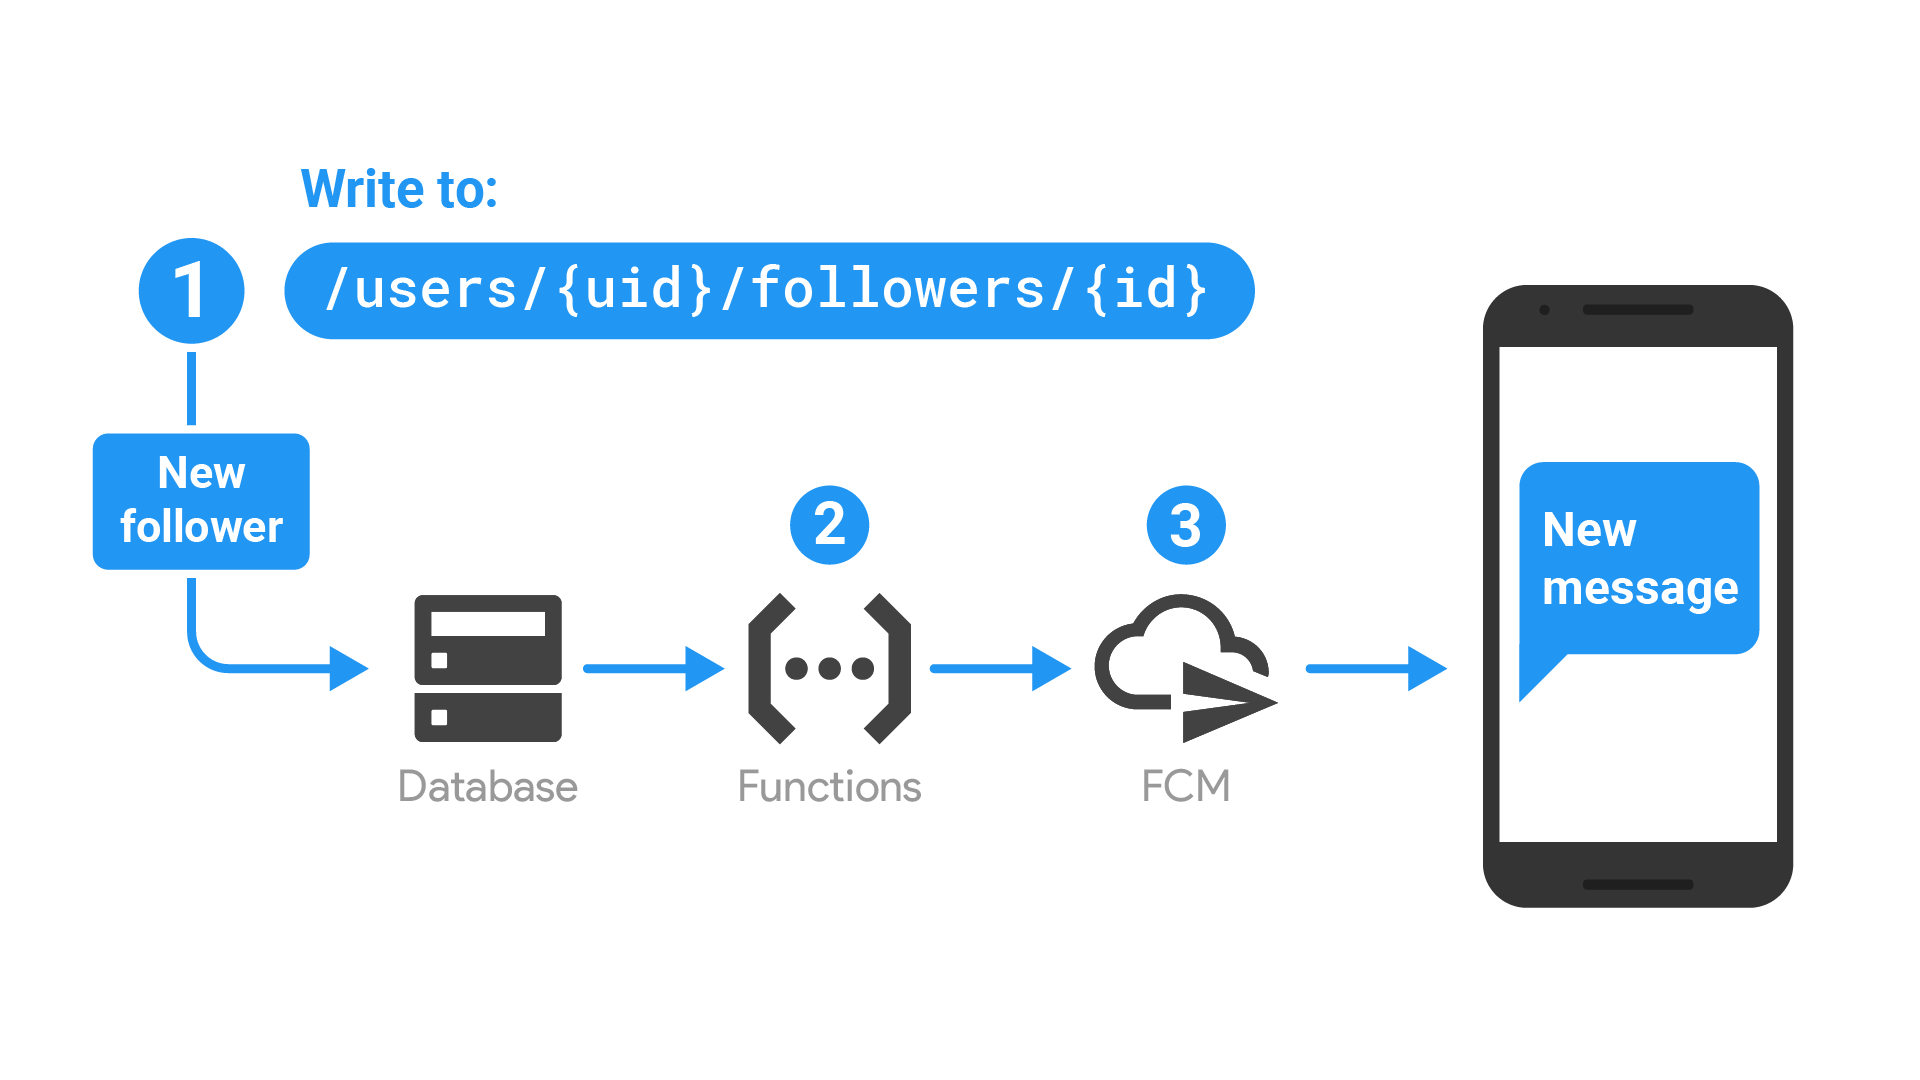
\includegraphics[scale=0.2]{images/firebase_functions_notify.png}
	\end{center}
	\caption{Cloud Functions Anwendungsfall Benachrichtigung}
	\label{fig:functions_notifications}
\end{figure}
In Abbildung \ref{fig:functions_notifications} ist ein typischer Anwendungsfall beschrieben. 
Ein Event auf der Datenbank wird ausgelöst, hier ein neuer Nutzer folgt einem weiteren Nutzer.
Es wird also ein Dokument in der Unter-Sammlung \texttt{followers} erzeugt. Diese Unter-Sammlung befindet sich innerhalb des Dokumentes \texttt{uid} der Sammlung \texttt{users}.
Im zweiten Schritt erstellt die Funktion eine Nachricht, welche über Firebase Cloud Messaging (FCM) versendet werden soll.
Über abgespeicherte Tokens sendet FCM die Benachrichtigung an das Gerät des Nuters \texttt{uid}.\cite{firebase2021}
\subsubsection{Cloud Messaging}
Firebase Cloud Messaging ist eine plattformübergreifende Messaging-Lösung zum zuverlässigen Versenden von Nachrichten an Nutzergeräte.
In Abbildung \ref{fig:cloudmessaging_architecture} ist die Architektur dieses Tools dargestellt.
Hierbei wird es grundlegend in das Erstellen, Transportieren und Empfangen der Nachrichten unterteilt.\cite{firebase2021}\\
\begin{itemize}
	\item \textbf{Erstellen} Die zu versendenden Nachrichten können, wie in Kapitel \ref{sec:cloudfunctions} beschrieben, manuell oder automatisiert erzeugt werden. 
	Bei der Automatisierung ist wichtig, dass die Nachrichten in einer vertrauenswürdigen Serverumgebung erstellt werden, damit alle Nachrichtentypen unterstützt werden (Schritt 1). 
	Das FCM Backend akzeptiert dann in Schritt 2 Nachrichtenanfragen, ordnet die Nachrichten verschiedenen Themen zu und erzeugt unter anderem Metadaten für Nachrichten, wie bspw. die Nachricht ID. 
	\item \textbf{Transportieren} Die Nachrichten werden hierbei an die entsprechenden Geräte weitergeleitet.
	Da verschiedene Geräte auf unterschiedlichen Plattformen basieren, muss die Transportschicht auf Plattformebene arbeiten.
	Hierfür werden folgende Ebenen genutzt:
	\begin{itemize}
		\item Android Transport Layer (ATL) für Android-Geräte mit Google Play-Diensten
		\item Apple Push Notification Service (APNs) für iOS-Geräte
		\item Web-Push-Protokoll für Web-Apps
	\end{itemize}
	\item \textbf{Empfangen} Das FCM SDK behandelt die Benachrichtigung oder Nachricht. Dies ist abhängig vom Vorder-/ Hintergrundstatus der Anwendung und der jeweiligen Anwendungslogik.
\end{itemize}


\begin{figure}[htb]
	\begin{center}
		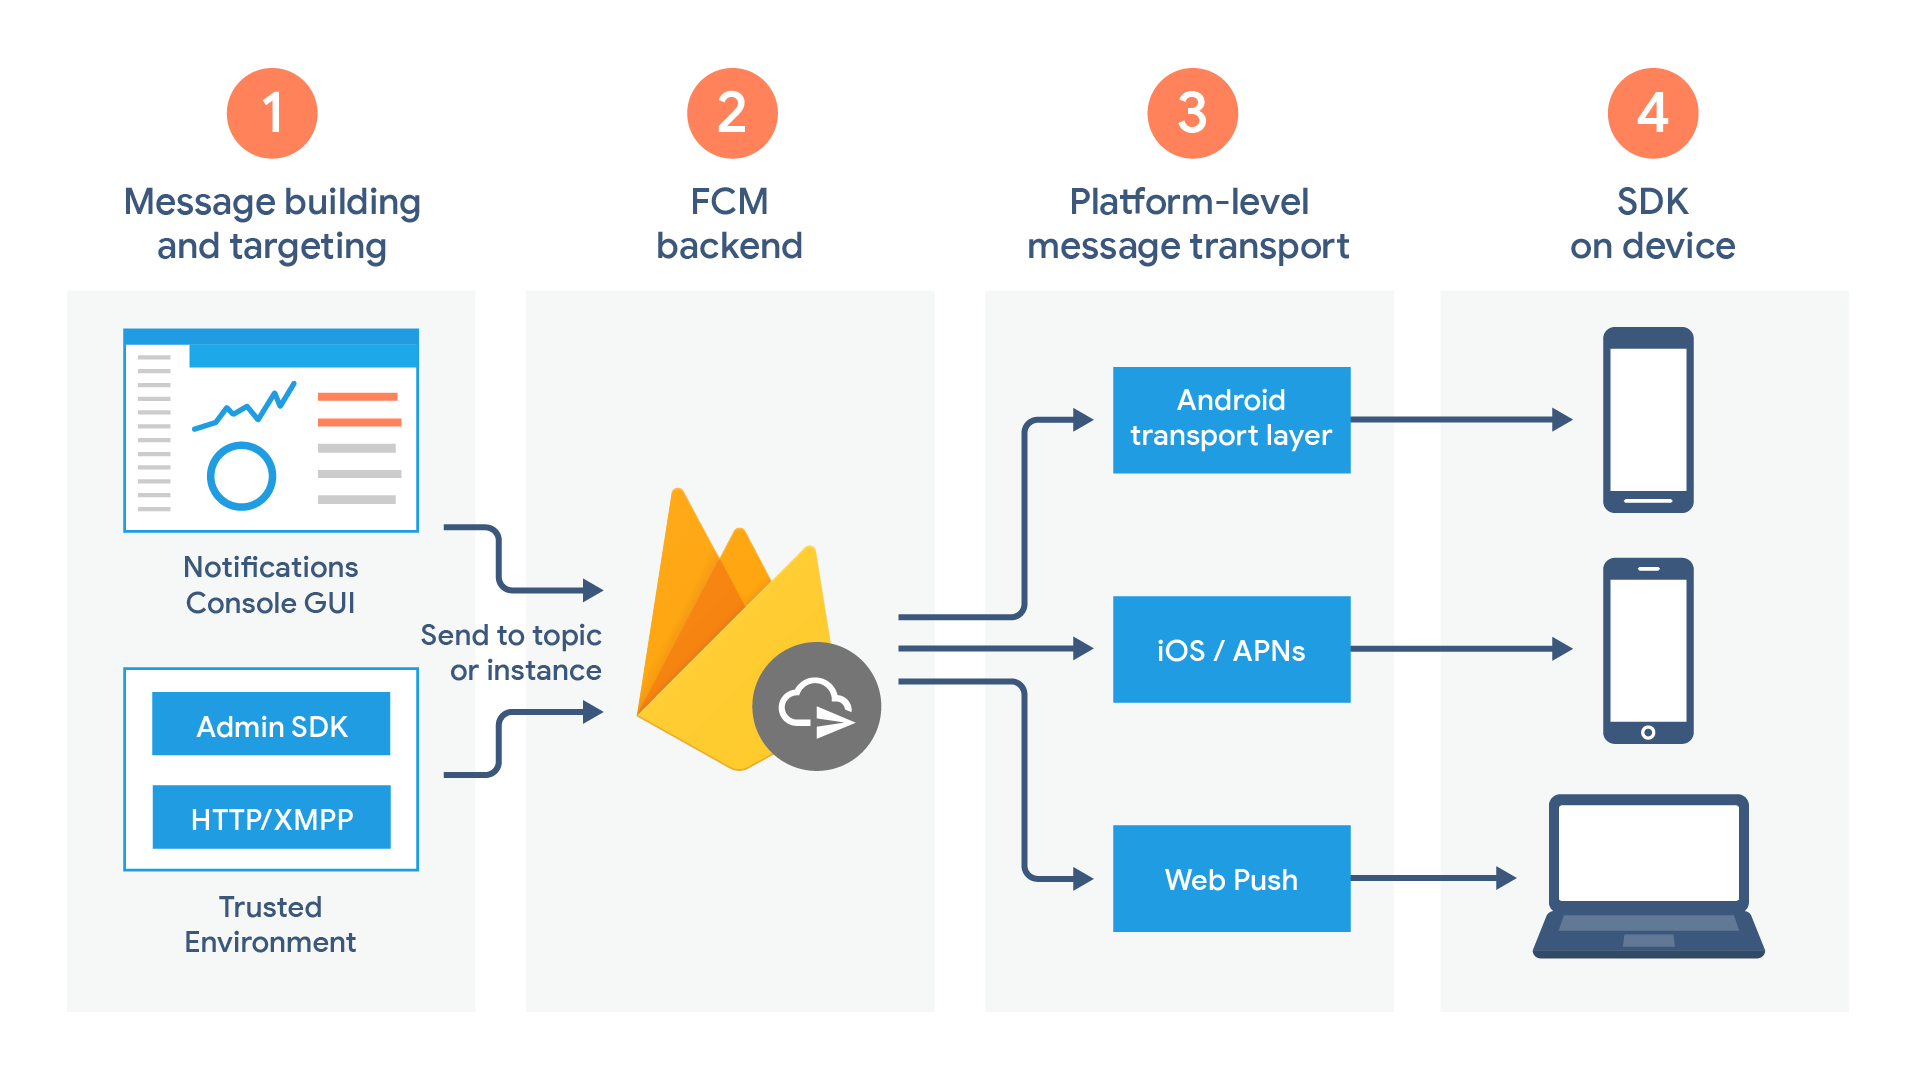
\includegraphics[scale=0.23]{images/firebase_cloudmessaging_architecture.png}
	\end{center}
	\caption{Firebase Cloud Messaging Architektur}
	\label{fig:cloudmessaging_architecture}
\end{figure}

\subsubsection{Google AdMob}
Google AdMob bietet eine einfache Art, gezielte Werbung innerhalb der Anwendung zu schalten und somit die Anwendung zu monetarisieren.
Zusätzlich bietet das Tool in Kombination mit Google Analytics\footnote{Ein freies Analysetool, welches über alle Tools hinweg Ereignisse sammelt und diese Werte direkt graphisch darstellt. Da es für die Implementierung nicht weiter relevant ist, wird es nicht detaillierter besprochen. Zusätzliche Informationen unter \href{https://firebase.google.com/docs/analytics}{firebase.google.com}.} zusätzliche Anwendungsdaten und Analysefähigkeiten.\\
Werbung lässt sich in unterschiedlicher Weise anzeigen (siehe Abbildung \ref{fig:firebase_admob})und lässt sich reibungslos in UI Komponenten integrieren. 
Verschiedene Features sind hier jedoch plattformabhängig. 
Auf der Android Plattform ist es für Nutzer möglich, beworbene Produkte direkt aus der Anwendung heraus zu kaufen.\\
Ein weiteres Werbetool \textit{Google Mobile Ads SDK} ist eine alleinstehende SDK, hingegen Google AdMob bietet einfache Integration in Firebase und weitere Tools.\cite{firebase2021}

\begin{figure}[htb]
	\begin{center}
		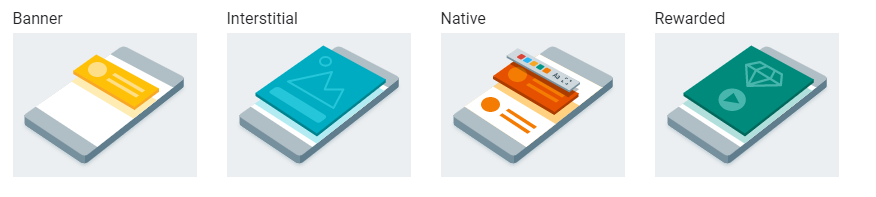
\includegraphics[scale=0.55]{images/firebase_admob_ads.PNG}
	\end{center}
	\caption{Google AdMob Anzeigemöglichkeiten}
	\label{fig:firebase_admob}
\end{figure}






































\subsection{Recommendationssystem}
Auf der Webseite Youtube allein werden minütlich mehr als 500 Stunden Videomaterial hochgeladen. (\url{https://blog.youtube/press/}, 10.02.2021)
Um bei einer solch unvorstellbaren Menge an Daten (allein auf einer Webseite) den Überblick als Endnutzer behalten zu können, ist ein personalisierten Filtersystems unausweichlich.

\noindent
Solche Filtersysteme, auch Recommendation System genannt, nutzt bisher gesammelte Daten um Nutzern potentiell interessante Objekte jeweils individuell vorzuschlagen.
Ein sogenannter \textit{Candidate Generator} ist hierbei ein Recommendation System, welches die Menge $M$ als Eingabe erhält und für jeden Nutzer eine Menge $N$ ausgibt. Hierbei umfasst $M$ alle Objekte und gleichzeitig gilt $N \subset M$. 

\noindent
Die Bestimmung einer solchen Menge $N$ beruht grundlegend auf zwei Informationsarten. Erstens die sogenannten Nutzer-Objekt Interaktionen, also beispielsweise Bewertungen oder auch Verhaltensmuster; Und zweitens die Attributwerte von jeweils Nutzer oder Item, also beispielsweise Vorlieben von Nutzern oder Eigenschaften von Items.\cite{aggarwal2016}
Systeme, welche zum Bewerten ersteres benutzen, werden \textit{collaborative filtering} Modelle genannt. Andere, welche zweiteres verwenden, werden \textit{content-based filtering} Modelle genannt. Wichtig hierbei ist jedoch, dass \textit{content-based filtering} Modelle ebenfalls Nutzer-Objekt Interaktionen (v.a. Bewertungen) verwenden können, jedoch bezieht sich dieses Modell nur auf einzelne Nutzer - \textit{collaborative filtering} basiert auf Verhaltensmustern von allen Nutzern bzw. allen Objekten.

\noindent
Ein solches Recommendation System kann im einfachsten Fall wie in \ref{Recommendation Matrix} als Matrix dargestellt werden.

\begin{table}[tbt]
	\caption{Nutzer-Item Matrix mit Bewertungen. Jede Zelle $r_{u;i}$ steht hierbei für die Bewertung des Nutzers $u$ an der Stelle $i$}
	\centering
	\label{Recommendation Matrix}
	\begin{tabular}{lcllllll}
		& \multicolumn{7}{c}{Items}                                                                                                                                                        \\
		& \multicolumn{1}{l}{}     & \multicolumn{1}{c}{1}  & \multicolumn{1}{c}{2}  & \multicolumn{1}{c}{...} & \multicolumn{1}{c}{i}  & \multicolumn{1}{c}{...} & \multicolumn{1}{c}{m}  \\ \cline{3-8} 
		& \multicolumn{1}{c|}{1}   & \multicolumn{1}{l|}{2} & \multicolumn{1}{l|}{}  & \multicolumn{1}{l|}{1}  & \multicolumn{1}{l|}{}  & \multicolumn{1}{l|}{}   & \multicolumn{1}{l|}{3} \\ \cline{3-8} 
		Users & \multicolumn{1}{c|}{2}   & \multicolumn{1}{l|}{4} & \multicolumn{1}{l|}{}  & \multicolumn{1}{l|}{}   & \multicolumn{1}{l|}{5} & \multicolumn{1}{l|}{}   & \multicolumn{1}{l|}{}  \\ \cline{3-8} 
		& \multicolumn{1}{c|}{...} & \multicolumn{1}{l|}{}  & \multicolumn{1}{l|}{}  & \multicolumn{1}{l|}{1}  & \multicolumn{1}{l|}{}  & \multicolumn{1}{l|}{}   & \multicolumn{1}{l|}{4} \\ \cline{3-8} 
		& \multicolumn{1}{c|}{u}   & \multicolumn{1}{l|}{}  & \multicolumn{1}{l|}{4} & \multicolumn{1}{l|}{}   & \multicolumn{1}{l|}{5} & \multicolumn{1}{l|}{}   & \multicolumn{1}{l|}{1} \\ \cline{3-8} 
		& \multicolumn{1}{l|}{}    & \multicolumn{1}{l|}{2} & \multicolumn{1}{l|}{}  & \multicolumn{1}{l|}{}   & \multicolumn{1}{l|}{}  & \multicolumn{1}{l|}{3}  & \multicolumn{1}{l|}{}  \\ \cline{3-8} 
		& \multicolumn{1}{l|}{n}   & \multicolumn{1}{l|}{}  & \multicolumn{1}{l|}{4} & \multicolumn{1}{l|}{}   & \multicolumn{1}{l|}{3} & \multicolumn{1}{l|}{}   & \multicolumn{1}{l|}{}  \\ \cline{3-8} 
	\end{tabular}
\end{table}

\subsubsection{Nutzerinformation}
Damit ein \textit{Recommender System} einem Nutzer Vorschläge bereitstellen kann, benötigt es Nutzerinformationen. Das Design des jeweiligen Systems hängt auch, wie oben beschrieben, von der Art der Information und von der Art der Beschaffung dieser ab.

\paragraph{Explizite Nutzerinformation}
Bei der expliziten Methode muss der Nutzer individuelle Informationen aktiv über sich preisgeben. Dies kann über konkrete Fragestellungen zu beispielsweise Geburtsdatum, Geschlecht oder Interessen geschehen. Diese Art der Information beschreiben einen Nutzer konkret. 

\noindent
Eine andere Art der Information sind Bewertungen von Objekten. Diese lassen sich beispielsweise Intervall basiert darstellen. Hierbei werden geordnete Zahlen in einem Intervall als Indikator genutzt, ob ein Objekt gut oder schlecht war - zum Beispiel eine Bewertung eines Produktes von 0 bis 5 Sternen bei Amazon. Diese Information beschreiben die Vorlieben eines Nutzers konkret.

\noindent
Je größer diese Skala ist, desto differenzierter ist auch das Meinungsbild, da jeder Nutzer sich genau ausdrücken kann. Jedoch desto komplizierter und unübersichtlich wird auch das Bewertungsverfahren an sich, da man einen zu großen Entscheidungsraum für den Nutzer darbietet.

\paragraph{Implizite Nutzerinformation}
Um implizit Nutzerinformationen zu erfassen, muss ein System die Verhaltensmuster seiner Kunden als Daten abspeichern. Beispielsweise könnte das System von YouTube erfassen, ob Videos frühzeitig abgebrochen oder ganz angeschaut werden. Anklicken von Webseiten und die darauf verbrachte Zeit könnte ebenfalls als Bewertung gespeichert und zur Generierung von Vorschlägen genutzt werden.

\subsubsection{Content-based filtering}
Unter \textit{content-based filtering} versteht man das Betrachten von Ähnlichkeiten zwischen Objekten anhand von Schlüsselwörtern (Eigenschaften) und daraus dann das Vorhersagen der Nutzer-Objekt Kombination für ein bestimmtes Objekt. 
Nimmt man an, Film 1 und Film 2 haben ähnliche Eigenschaften (gleiches Genre, gleiche Schauspieler, ...) und Nutzer A mag Film 1, so wird das System Film 2 vorschlagen.

\noindent
Das System ist also unabhängig von anderen Nutzerdaten, da die Vorschläge nur auf Präferenzen eines einzelnen Nutzers basieren. Dies bietet im Hinblick auf eine App auch gute Skalierungs"-möglich"-keiten. Zudem kann auf Nischen-Präferenzen gut eingegangen werden, da nicht mit anderen Nutzerdaten verglichen wird, sondern nur ein Nutzer für sich betrachtet wird.

\noindent
Gleichzeitig schlagen \textit{content-based filtering} Systeme aber eher offensichtliche Objekte vor, da Nutzer oft unzureichend genaue "Beschreibungen", also Vorlieben mit sich bringen. Dadurch, dass nur basierend auf Schlüsselwörter neue Objekte vorgeschlagen und andere Nutzerwertungen nicht miteinbezogen werden, sind die Vorschläge sehr wahrscheinlich oftmals ähnlich bis gleich - man "verfängt" sich quasi in eine Richtung.\cite{aggarwal2016}

\subsubsection{Collaborative Filtering}
Unter \textit{collaborative filtering} versteht man das Betrachten von Ähnlichkeiten im Verhalten von Nutzern anhand von Bewertungen und Prä"-fer"-enzen, bzw. anhand der Ähn"-lich"-keiten von Objekten.

\noindent
Generell unterscheidet man in zwei Typen:\cite{aggarwal2016}

\begin{enumerate}		
	\item \textit{Memory-based Methoden}: Es wird, wie oben beschrieben, aus gesammelten Daten Ähn"-lich"-keit herausgearbeitet und Nutzer-Objekt Kombinationen durch eben diese vorhergesagt. Daher wird dieser Typ auch \textit{neighborhood-based collaborative filtering} genannt. Man unterscheidet weiter in:
	\begin{enumerate}
		\item \textit{User-based}: Ausgehend von einem Nutzer A werden andere Nutzer mit ähnlichen Nutzer-Objekt Kombinationen gesucht, um Vorhersagen für Bewertungen von A zu treffen. Ähnlichkeitsbeziehungen werden also über die Reihen der Bewertungsmatrix berechnet.
		\item \textit{Item-based}: Hierbei werden ähnliche Objekte gesucht und diese genutzt um die Bewertung eines Nutzers für ein Objekt vorherzusagen. Es werden somit Spalten für die Berechnung der Ähnlichkeitsbeziehungen verwendet.
	\end{enumerate}
	\item \textit{Model-based Methoden}: Machine Learning und Data Mining Methoden werden verwendet um Vorhersagen über Nutzer-Objekt Kombinationen zu treffen. Hierbei sind auch gute Vorhersagen bei niedriger Bewertungsdichte in der Matrix möglich.
\end{enumerate}

\noindent
Vereinfacht gesagt: Wenn Nutzer A ähnliche Bewertungen verteilt wie Nutzer B, und B den Film 1 positiv bewertet hat, wird das System Film 1 auch Nutzer A vorschlagen. Das selbe gilt auch umgekehrt (\textit{Item-based}).

\noindent
Diese Art leidet sehr unter dem \textit{sparsity} Problem, also dass die Nutzer zu wenige Bewertungen von Objekten ausüben. Daher sind Vorhersagen über Ähnlichkeit von Nutzern aufgrund unzureichender Datensätze nicht sinnvoll möglich. Dieses Problem wird \textit{Cold-Start Problem} genannt.

\subsubsection{Ähnlichkeit von Objekten und Nutzern}
Sowohl bei \textit{collaborative filtering}, als auch bei \textit{content-based filtering} wird jedes Objekt und jeder Nutzer als ein Vektor im Vektorraum-Modell $E = \mathbb{R}^d$ (englisch \textit{embedding space}) erfasst. Sind Objekte beispielsweise ähnlich, haben sie eine geringe Distanz voneinander. 

\noindent
Ähnlichkeitsfunktionen sind Funktionen $s : E \times E  \rightarrow \mathbb{R}$ welche aus zwei Vektoren beispielsweise von einem Objekt $q \in E$ und einem Nutzer $x \in E$ ein Skalar berechnen, welches die Ähnlichkeit dieser zwei beschreibt $s(q,x)$.

\noindent
Hierfür werden mindestens eine der folgenden Funktionen verwendet:
\begin{itemize}
	\item Cosinus-Funktion
	\item Skalarprodukt
	\item Euklidischer Abstand
\end{itemize} 

\paragraph{Cosinus-Funktion}
Hier wird einfach der Winkel zwischen beiden Vektoren berechnet: $s(q,x) = \cos(q,x)$

\paragraph{Skalarprodukt}
Je größer das Skalarprodukt, desto ähnlicher sind sich die Vektoren. $s(q,x) = q \circ x = \sum_{i=1}^{d}q_i x_i$ 

\paragraph{Euklidischer Abstand}
$s(q,x) = ||q-x|| = [\sum_{i=1}^{d}(q_i - x_i)^2]^\frac{1}{2}$





\url{https://dl.acm.org/doi/pdf/10.1145/3383313.3412488}
\url{http://www.microlinkcolleges.net/elib/files/undergraduate/Photography/504703.pdf}	
		
\section{Konzept?}
\label{sec:app_concept}
%TODO Section{Idee/Gedankengänge/Planung} in der \subsectino{Konzept} mit den Wünschen des Users und die Benötigten Ressourcen und eine subsection{Komponenten} mit Unseren Komponenten/Ressourcen und wie sie miteinander funktionieren.

\subsection{Konzept}
Aus Perspektive der Benutzer ist die Idee hinter StreamSwipe trivial. Dem User werden nacheinander Filme und Serien vorgeschlagen, die er bewerten kann. Auf Basis seiner Präferenzen erhält er Matches, mit denen er über sich eine Chatfunktionen austauschen kann. Jeder dieser Schritte muss möglichst schnell und unkompliziert erfolgen.\\
Aus Sicht des Anbieters ist die Realisierung wesentlich komplexer als es dem User erscheint, da eine Zusammenstellung an Komponenten benötigt wird.  Diese besteht aus einer Smartphone-App, einer Userdatenbank, einer Datenbank mit den Filminformationen und einem Server, der das Matching ausführt. Zusätzlich wird eine mögliche Komponente für den Messenger benötigt. Die Auswahl dieser Komponente wird jeweils über individuell gestellte Anforderungen getroffen. \\

\noindent
Bei der Smartphone-App muss bereits während der Entwicklung auf Benutzerfreundlichkeit und Barrierefreiheit geachtet werden. Sie sollte intuitiv bedienbar, attraktiv designt und ressourcensparend für leistungsschwache Smartphones programmiert sein. Um ein möglichst großes Publikum ansprechen zu können, muss sie für iOS und Android erhältlich sein.\\
Die Datenbank mit den Benutzerinformationen muss jederzeit erreichbar sein und eine gewisse Form von Sicherheit und Verschlüsselung bieten, da da hier persönliche Angaben gespeichert werden.\\
Die Datenbank mit den Filminformationen  muss sehr umfangreich sein, also auch ältere Filme und Nischenfilme enthalten, und ständig aktualisiert werden. Neben den offensichtlichen Informationen wie Filmtitel und Filmposter muss sie auch weitere Daten zu den Filmen enthalten wie Erscheinungsdatum, Handlung, Regie, etc. trotzdem sollte der Zugriff schnell sein und nichts kosten, sodass die Nutzung der App möglichst preiswert ist.\\
Der Server muss durchgehend laufen und über eine Internetverbindung erreichbar sein. Er muss leistungsstark genug sein um alle Nutzeranfragen bedienen zu können, sollte jedoch so klein gehalten werden, dass die Anschaffungs- und Unterhaltskosten minimal sind.\\
Der Messenger  muss ebenfalls über einen zentralen Punkt gesteuert werden, da sich nur zwischen Personen ein Chat öffnen darf, die gematcht wurden. Es sollte keine Zugriffsbegrenzung auf diesen Server  geben, um einen unbegrenzten  Nachrichtenwechsel garantieren zu können. Nachrichten müssen gespeichert werden, um versendete Nachrichten auch nach dem Schließen der App zustellen zu können. Das System muss ebenfalls verschlüsselt sein und benötigt Zugriff auf Benutzerinformationen wie ID, Name und Profilbild.



X Server muss ständig laufen/erreichbar sein und Internetverbindung haben. In diesem Fall ein Raspberry Pi mit ... was eigentlich??? \\ %TODO Kapitel lesen!!!



\subsection{Komponenten}
\label{sec:komponenten}
In StreamSwipe ist für jede dieser Komponenten eine Lösung gefunden worden.
Bei der Entwicklung der App wurden Benutzerfreundlichkeit und Barrierefreiheit beachtet, wie in Abschnitt \ref{sec:UI-allgemein}, bzw. Abschnitt \ref{sec:barrierefreiheit} gezeigt wird. Wie in Abschnitt \ref{sec:framework} beschrieben wird, können die genannten Anforderungen durch eine geschickte Wahl des Frameworks erfüllt werden. Als Benutzerdatenbank kann Firebase verwendet werden, da wie in Abschnitt \ref{sec:firebase} beschrieben, die benötigten Funktionen vorhanden sind. Es ist ebenfalls möglich den Messenger mit den Firebasefunktionen zu implementieren. Als Quelle der Filminformationen wird die API von \glqq The Movie Database\grqq \, (TMDb) verwendet, auf welche in Abschnitt \ref{sec:filmdatenbank} genauer eingegangen wird. Der verwendete Server besteht aus einem Raspberry Pi, jedoch mehr dazu in Kapitel \ref{sec:server}. Wie diese Komponenten aufeinander zugreifen wird in Abbildung \ref{fig:komponentendiagramm} verdeutlicht.\\
Über die Smartphone-App werden die Benutzerdaten an Firebase weitergeleitet. Wird ein neuer Account angelegt, so werden diese Daten dort gespeichert und bei einem Anmeldevorgang sie mit den bestehenden Benutzerdaten verglichen. Nur wenn der User bereits vorhanden ist, kann eine Anmeldung stattfinden. So wird sichergestellt, dass nur angemeldete Benutzer auf die eigentlichen Funktionen der App Zugriff erhalten. Jede Aktion in der App wird auf diese Weise einem Benutzerkonto zugewiesen und kann später darüber identifiziert werden. Innerhalb der App können alle Funktionen frei genutzt werden weshalb es wichtig ist, dass ausschließlich eingeloggte User auf die Screens der App zugreifen können.\\
Der Server erhält die Film-IDs aller Filme aus der TMDb-API  und erstellt somit eine eigene Film-Datenbank. Diese IDs werden an das Smartphone weitergeleitet und die App erhält über die IDs die Filminformationen direkt von der TMDb-API. Es werden gleichzeitig nur eine geringe Anzahl an Filminformationen aus der TMDb-API auf das Smartphone geladen, sodass dieser Vorgang möglichst wenig Ressourcen benötigt und unbemerkt im Hintergrund ablaufen kann. Hierzu zählen Filmposter, Rating, Besetzung, Veröffentlichungsdatum, übersetzte Sprachen und viele mehr, die teilweise nicht benötigt werden. Noch bevor der User über alle diese Filme abgestimmt hat, werden neue Filminformationen geladen, sodass es für den User keine Unterbrechungen gibt und es ihm wie ein einzelner unendlicher Fluss an Daten erscheint. \\
Die Filmbewertung wird mit den Film-IDs vom Smartphone an den Server geschickt, der diese beiden Informationen miteinander verknüpft. Das Rekommendationsverfahren auf dem Server verarbeitet diese Präferenzen und sucht wie in Kapitel \ref{sec:recomandationSystem} beschrieben nach Übereinstimmungen bei den anderen Benutzern. Da hierbei alle Präferenzen aller User miteinander verglichen werden, ist dieser Schritt sehr aufwändig und sollte nicht nach jeder neuen Präferenz durchgeführt werden. Bei StreamSwipe wird dieses Matching deshalb automatisch in regelmäßigen Zeitabständen durchgeführt, optimalerweise zu einer Tageszeit, an der die Benutzeraktivität gering ist. Die Anzahl der verglichenen Nutzer kann mit einer Filterung durch Geschlechterpräferenzen und Wohnort reduziert werden um das Matchingverfahren zu beschleunigen. \\
Werden zwei User gematcht, wird dies ihnen jeweils in der App angezeigt. Die beiden Benutzer können dann einzeln entscheiden, ob sie die Unterhaltung starten wollen. Ist dies der Fall, werden die Nachrichten in der Firebase-Datenbank gespeichert. %TODO hier die abläufe des chats abklären!!!



%TODO Auch Leon fragen wie exakt das ganze abläuft
- Der Messenger kann ebenfalls über Firebase realisiert werden\\ %TODO Inwieweit gibts hier ein Kapitel drüber?

- Nutzer ID von beiden Nutzern bekannt bei der  Erstllung eines Chats
- Aus diesen beiden wird eine unique ID für den jeweiligen Chat erstellt und diese wird bei beiden Usern gespeichert
- (Firebase ist hierarchisch aufgebaut) Nutzernamen, NutzerID und RoomID werden in einer Sammlung gespeichert. Unter dieser Sammlung werden dann die Nachrichten abgespeichert mit den Informationen Wers gesendet hat, wers empfängt, einen tmestamp und natürlcih den inhalt der nachricht. sendby und sendto werden verwendet um die nachrichten im Chatverlauf anzuordnen und zu entscheiden welcher der beiden beteiligten eine benachrichtigung bekommt
- Anzeige der Chats abhängig davon ob die uniqueID in chatrooms oder pendingchatrooms gespeichert ist
- Wer die unterhaltung beginnt, erhält die unique ID in chatrooms und der andere in pendingchatrooms
- NImmt der andere User den Chat an, wird die ID für ihn ebenfalls in chtarooms verschioben
-


\begin{figure}[h]
\centering
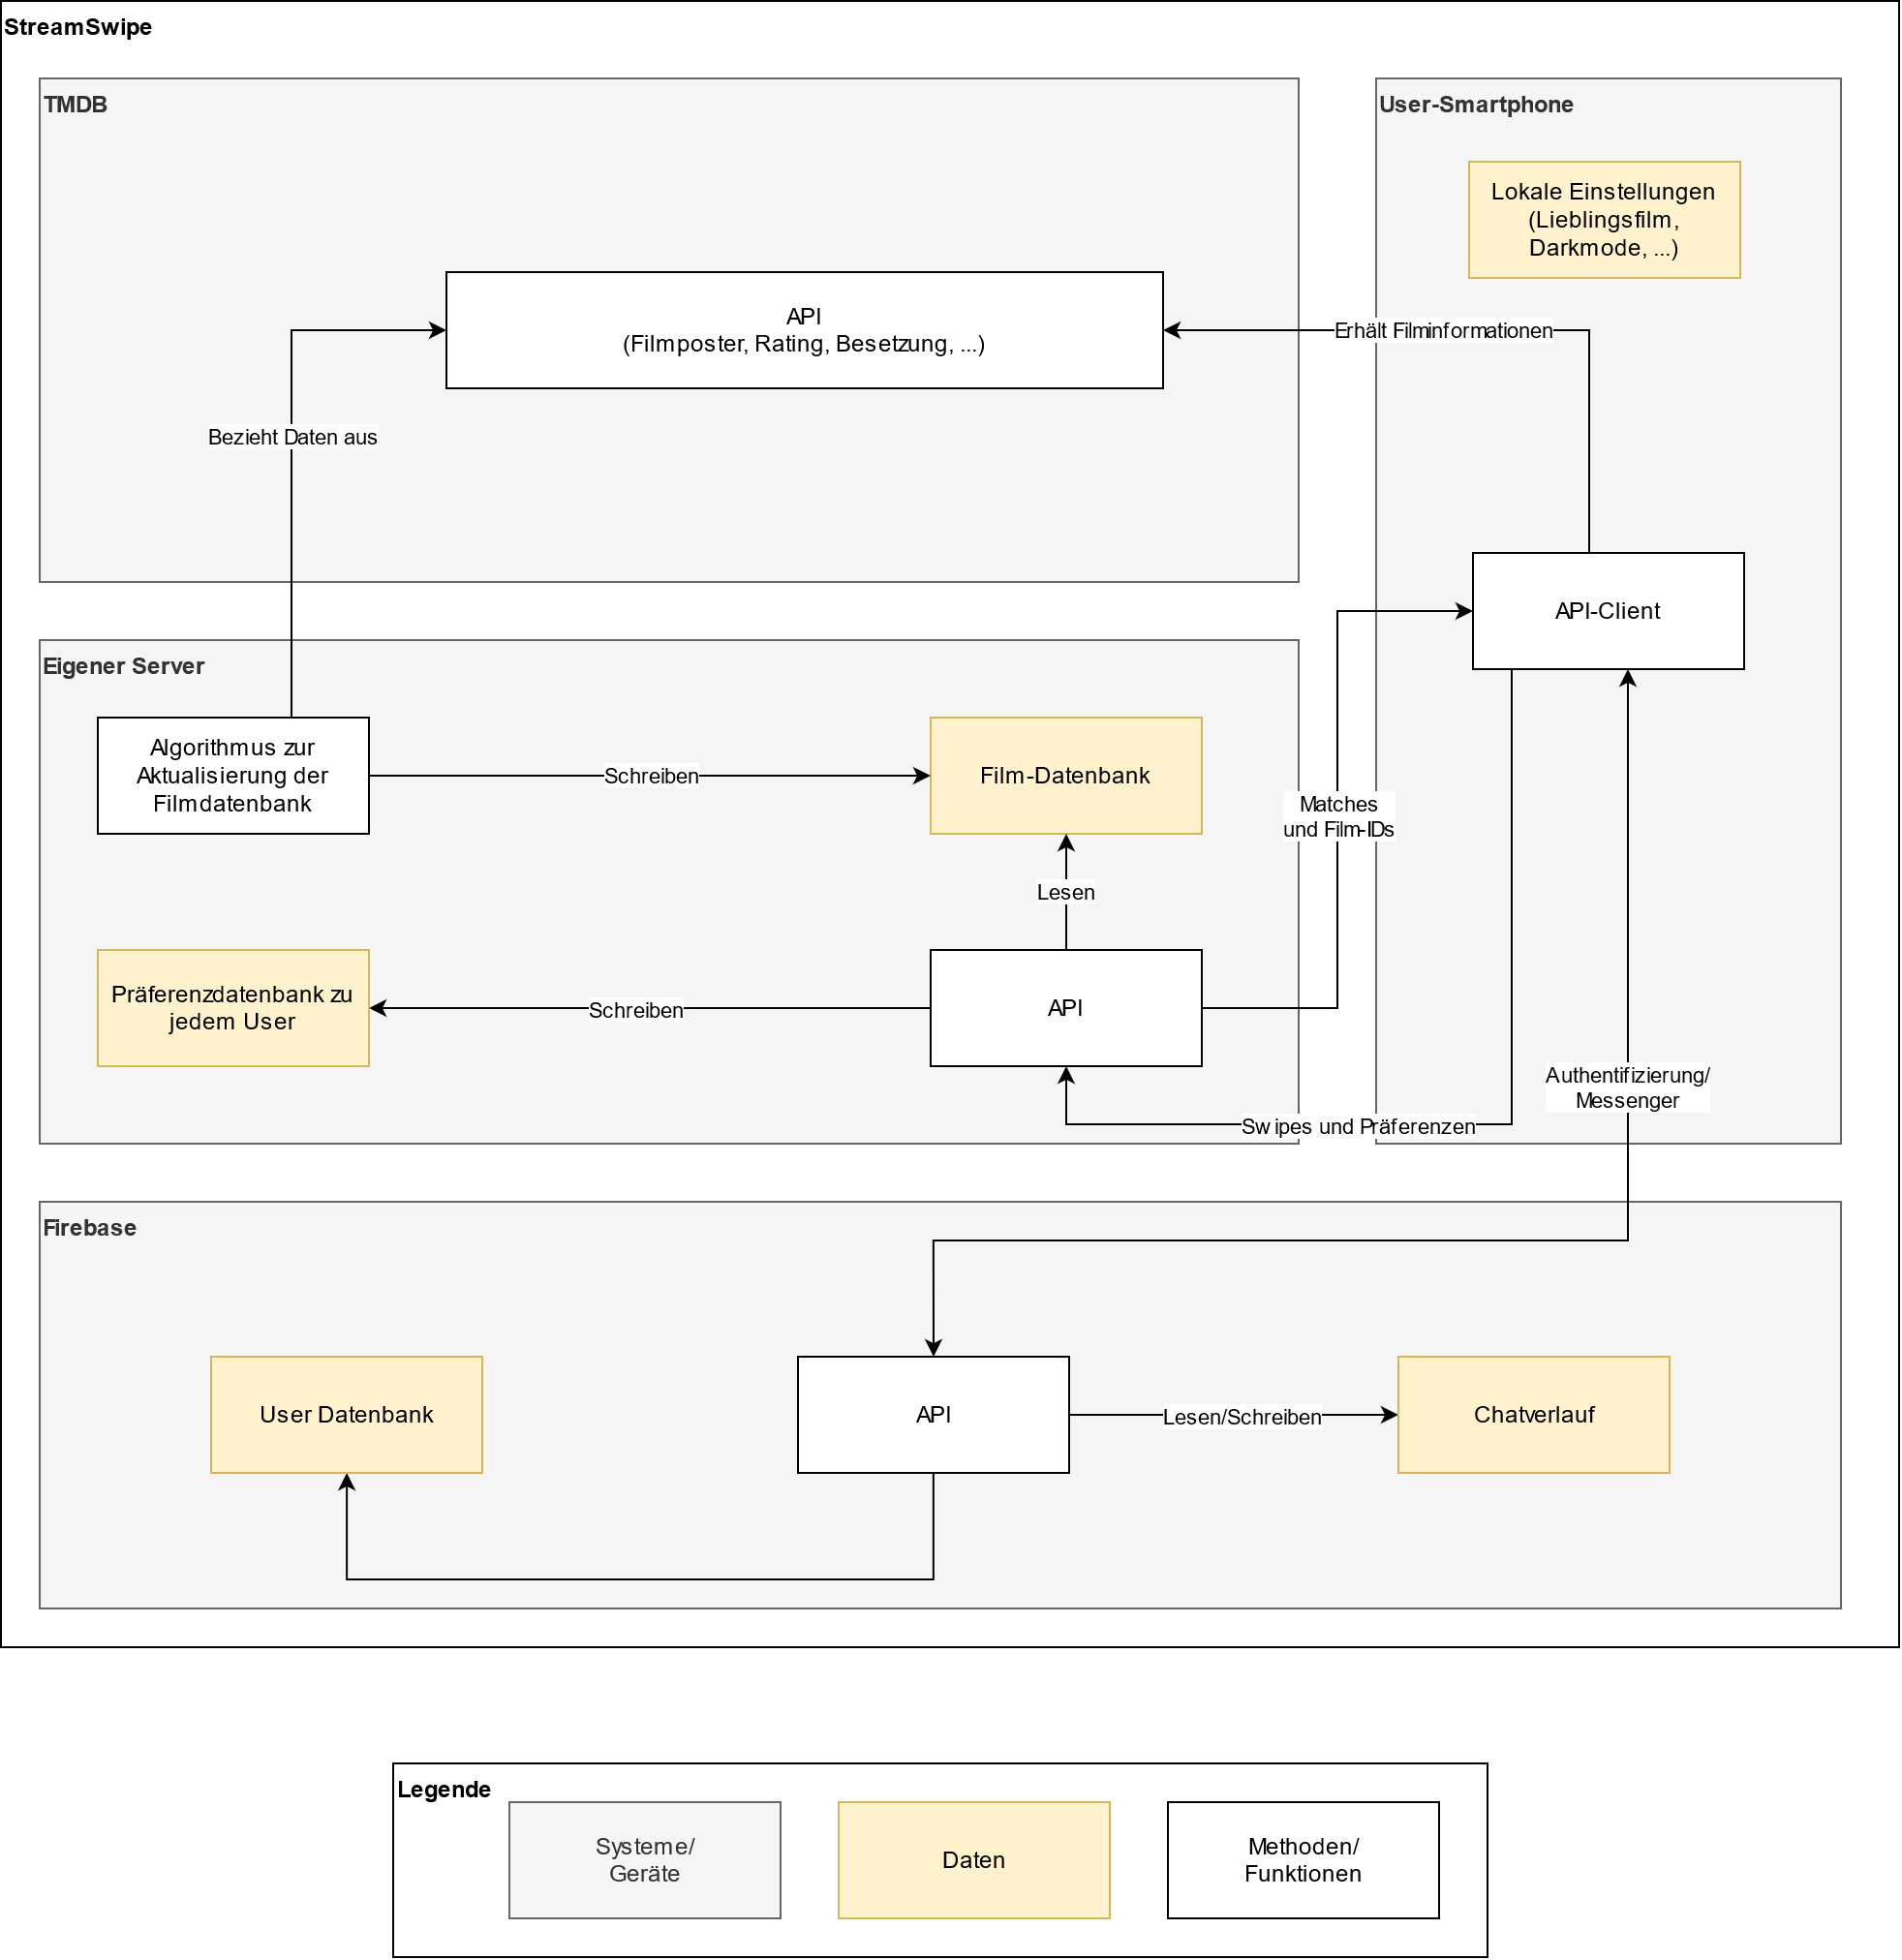
\includegraphics[width=16cm]{images/Konzeptdiagramm.png}
\caption{Komponentendiagramm}
\label{fig:komponentendiagramm}
\end{figure}

\section{Funktionen/Komponenten}

\subsection{Swipe/Aussuchen/Voting}		
\subsection{Matches/Chat}		
\subsection{Film-/Serienvorschläge}		
\subsection{Gruppenorgien}		
\subsection{Gespeicherte Filme/Filmliste}		
\subsection{Zugänglichkeit/Behindertenfreundlichkeit}		


\section{Benutzeroberflächen}
\subsection{Home-Screen}
\subsection{Gruppen}		
\subsection{Chat}		
\subsection{Filmliste}

\section{CodeBeispiele}


\section{Probleme}


\section{Fazit}

\end{document}



\footnote{\url{https://de.wikipedia.org/wiki/Alufolie}} 


Abbildung \ref{fig:allg_kennlinie}

\begin{figure}[tbt]
\begin{center}
\includegraphics[scale=0.45]{Grafiken/allg_kennlinie.png}
\end{center}
\caption{Kennlinie einer Halbleiterdiode \protect \footnotemark}
\label{fig:allg_kennlinie}
\end{figure}
\footnotetext{FUSSNOTE}


Tabelle \ref{tab:cobalt}

\begin{table}[tbt]
\caption{•}
\begin{threeparttable}	%Scheme for footnotes in tables
\begin{center}
\begin{tabular}{c c c c}
\toprule
& keV & keV & keV \\
\midrule
a	& b	& c	& d \\
a	& b	& c	& d \\
a	& b	& c	& d \\
a	& b	& c	& d \\ %direkt hinter jeweiligen Wert /tnote{1}
\bottomrule
\end{tabular}
\end{center}
\begin{tablenotes}\footnotesize 
\item[1]{Quelle: http://www.thinksrs.com/downloads/PDFs/ApplicationNotes/IG1BAgasapp.pdf}
\end{tablenotes}
\end{threeparttable}
\label{tab:cobalt}
\end{table}